% ***********************************************************
% ******************* PHYSICS HEADER ************************
% ***********************************************************
% Version 2
\documentclass[12pt]{article}
\usepackage{amsmath} % AMS Math Package
\usepackage{amsthm} % Theorem Formatting
\usepackage{amssymb}    % Math symbols such as \mathbb
\usepackage{graphicx} % Allows for eps images
\usepackage[dvips,letterpaper,margin=1in,bottom=0.7in]{geometry}
%\usepackage{tensor}
 % Sets margins and page size
\usepackage{amsmath}
\usepackage{caption}
\usepackage{subcaption}

\renewcommand{\labelenumi}{(\alph{enumi})} % Use letters for enumerate
% \DeclareMathOperator{\Sample}{Sample}
\let\vaccent=\v % rename builtin command \v{} to \vaccent{}
\usepackage{enumerate}
\renewcommand{\v}[1]{\ensuremath{\mathbf{#1}}} % for vectors
\newcommand{\gv}[1]{\ensuremath{\mbox{\boldmath$ #1 $}}} 
% for vectors of Greek letters
\newcommand{\uv}[1]{\ensuremath{\mathbf{\hat{#1}}}} % for unit vector
\newcommand{\abs}[1]{\left| #1 \right|} % for absolute value
\newcommand{\avg}[1]{\left< #1 \right>} % for average
\let\underdot=\d % rename builtin command \d{} to \underdot{}
\renewcommand{\d}[2]{\frac{d #1}{d #2}} % for derivatives
\newcommand{\dd}[2]{\frac{d^2 #1}{d #2^2}} % for double derivatives
\newcommand{\pd}[2]{\frac{\partial #1}{\partial #2}} 
% for partial derivatives
\newcommand{\pdd}[2]{\frac{\partial^2 #1}{\partial #2^2}} 
% for double partial derivatives
\newcommand{\pdc}[3]{\left( \frac{\partial #1}{\partial #2}
 \right)_{#3}} % for thermodynamic partial derivatives
\newcommand{\ket}[1]{\left| #1 \right>} % for Dirac bras
\newcommand{\bra}[1]{\left< #1 \right|} % for Dirac kets
\newcommand{\braket}[2]{\left< #1 \vphantom{#2} \right|
 \left. #2 \vphantom{#1} \right>} % for Dirac brackets
\newcommand{\matrixel}[3]{\left< #1 \vphantom{#2#3} \right|
 #2 \left| #3 \vphantom{#1#2} \right>} % for Dirac matrix elements
\newcommand{\grad}[1]{\gv{\nabla} #1} % for gradient
\let\divsymb=\div % rename builtin command \div to \divsymb
\renewcommand{\div}[1]{\gv{\nabla} \cdot \v{#1}} % for divergence
\newcommand{\curl}[1]{\gv{\nabla} \times \v{#1}} % for curl
\let\baraccent=\= % rename builtin command \= to \baraccent
\renewcommand{\=}[1]{\stackrel{#1}{=}} % for putting numbers above =
\providecommand{\wave}[1]{\v{\tilde{#1}}}
\providecommand{\fr}{\frac}
\providecommand{\RR}{\mathbb{R}}
\providecommand{\NN}{\mathbb{N}}
\providecommand{\seq}{\subseteq}
\providecommand{\e}{\epsilon}

\newtheorem{prop}{Proposition}
\newtheorem{thm}{Theorem}[section]
\newtheorem{axiom}{Axiom}[section]
\newtheorem{p}{Problem}[section]
\usepackage{cancel}
\newtheorem*{lem}{Lemma}
\theoremstyle{definition}
\newtheorem*{dfn}{Definition}
 \newenvironment{s}{%\small%
        \begin{trivlist} \item \textbf{Solution}. }{%
            \hspace*{\fill} $\blacksquare$\end{trivlist}}%
% ***********************************************************
% ********************** END HEADER *************************
% ***********************************************************

\begin{document}

{\noindent\Huge\bf  \\[0.5\baselineskip] {\fontfamily{cmr}\selectfont  Problem Set I}         }\\[2\baselineskip] % Title
{ {\bf \fontfamily{cmr}\selectfont Methods of Molecular Simulations}\\ {\textit{\fontfamily{cmr}\selectfont     April  21, 2021}}}~~~~~~~~~~~~~~~~~~~~~~~~~~~~~~~~~~~~~~~~~~~~~~~~~~~~~~~~~~~~~~~~~~~~~~~~~~~~~    {\large \textsc{Mahesh Yadav}\footnote{With }} % Author name
\\[1.4\baselineskip] 



\section{Hamiltonian dynamics}
%\emph{Some materials have a property called "optical activity,” that is, for circularly     polarized light, their index of refraction (and therefore their wavelength in the medium) depends on whether the light is right- or left-circularly polarized. The EM waves propagating in the $+\uv{z}$ direction inside such a medium can therefore be described by}


\begin{p} The motion of mass m = 1 g connected to a harmonic spring with spring constant $k = 0.1 N/m$ is governed by the canonical equations
\begin{equation}
   \dot{x}(t) = p(t) / m, \; \; \; \; \; \; \dot{p}(t) = -kx(t)
\end{equation}
where $x(t)$ denotes the displacement from the equilibrium position at time $t$ and $p(t)$ the momentum. Solve this set of linear differential equations numerically using $(i)$ Heun's method (i.e., the explicit midpoint method), and $(ii)$ the velocity-Verlet algorithm. 
\bigbreak
 a) Consider time from $t=0 $ to 10 seconds and timesteps $\delta t = 10^{-3}s $ and $10^{-1}s$ with the initial conditions $x(0)=0 $ and $p(0)=10^{-3} kg. m/s $. Plot your numerical solutions as a function of time and compare with the analytical results. Plot the trajectories in phase space, i.e., momentum $p(t) $ vs. displacement $x(t) $. Discuss your results. \\
 \vskip 0.1in
 b) Calculate the numerically obtained total energy $E(t)$ and plot the deviation $\Delta E(t) := E(t) - E(0)$ for the previous results. Also plot $\Delta E(t) / \Delta t$ and $\Delta E(t) / (\Delta t)^2$ for the different timesteps. Which algorithm would you suggest for molecular dynamics simulations?\\
 \vskip 0.1in
 c*) Determine the corresponding Liouville operator. Express both integration algorithms by splitting formulas and argue that Heun's method is not invariant under time reversal $(t \rightarrow -t, v \rightarrow -v)$. Test this numerically by reverting the integration.

\end{p}
\begin{s} \underline{\bf{Heun's method}} \par
Heun's method is the extension of the Euler's method. The problem with the simple Euler method is that the derivative at the beginning of the interval is assumed constant over the entire step; the derivative at the end of interval is not used. Such asymmetric treatments always lead to low levels of accuracy in the solution. \par
The basic idea behind Heun's method using a prediction line whose slope is the average of the slopes of the tangents lines at either end of the interval. The iteration formulas for the Heun's method are,
%
\begin{equation}
x_{n+1} = x_{n} + h
\end{equation}
%
%
\begin{equation}
y_{n+1} = y_{n} + \frac{h}{2} (f(x_{n}, y_{n}) + f(x_{n} + h, y_{n} + h f(x_{n}, y_{n})))
\end{equation}
%
In the scenario of a mass connected to a harmonic spring the function $f$ is defined as
\begin{equation}
	f(t,y) = 
	\begin{bmatrix}
		\frac{y_2(t)}{m} \\
		-ky_1 (t)
		\end{bmatrix}
\end{equation}
with given initial values $y_1 (0) = 0$ and $y_2 (0) = 0.001$, mass $m=0.001$ kg and spring constant $k=0.1 N/m$. In the following observations the time interval is set from $t=0$ to $t=10s$ with altered step sizes h.
In figure 1, Heun's method for a mass connected to a harmonic spring is compared to the analytical solution. For a step size $h=0.001$ is the numerical approximation equal to the analytical solution. However, by decreasing the step size Heun's method rapidly leaves the ellipse, see subfigure b) and c)
%
\begin{figure}[!h]
	\center{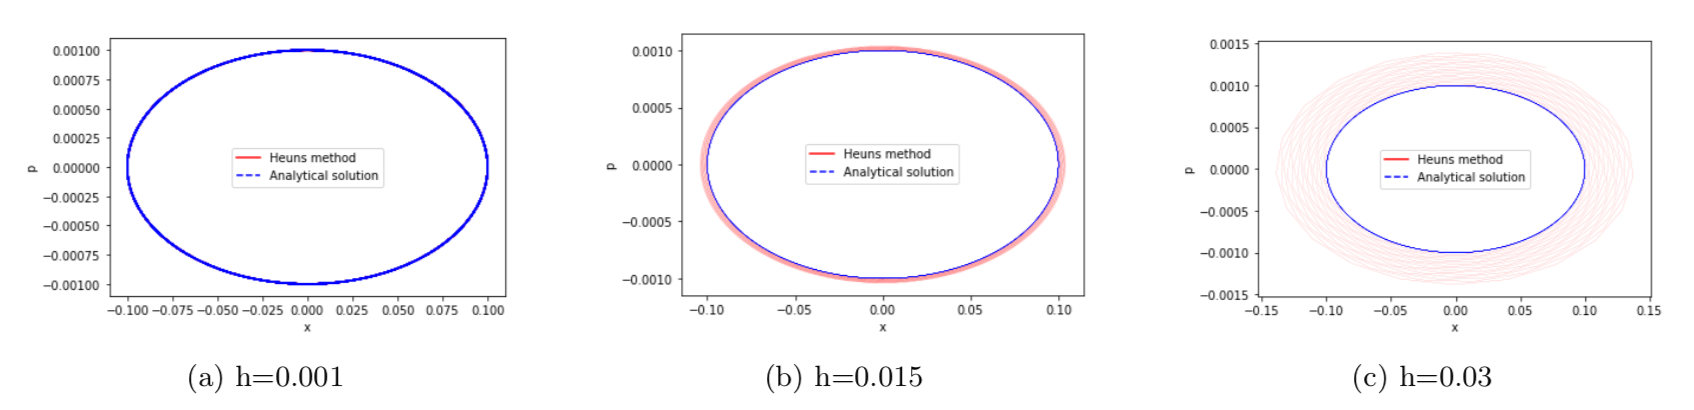
\includegraphics[width=18cm]{pic1.png}}
	\caption{\label{fig:my label} Heun's method compared to analytical solution for different step sizes.}
\end{figure}
%
The energy of the system can be calculated by
%
\begin{equation}
	E(t) = \frac{p(t)^2} {2m} + \frac{kx(t)^2} {2}
\end{equation}
%
The numerically obtained energy of the system using Heun's method is not conserved (figure 2). Further, the energy deviation is rapidly growing with increasing step sizess. Comparing the energy deviation with the plots in 3 and 4, the deviation scales linear with the different timesteps. Thus the velocity-verlet algorithm should be used for molecular dynamics simulations. 
%
\begin{figure}[!h]
	\center{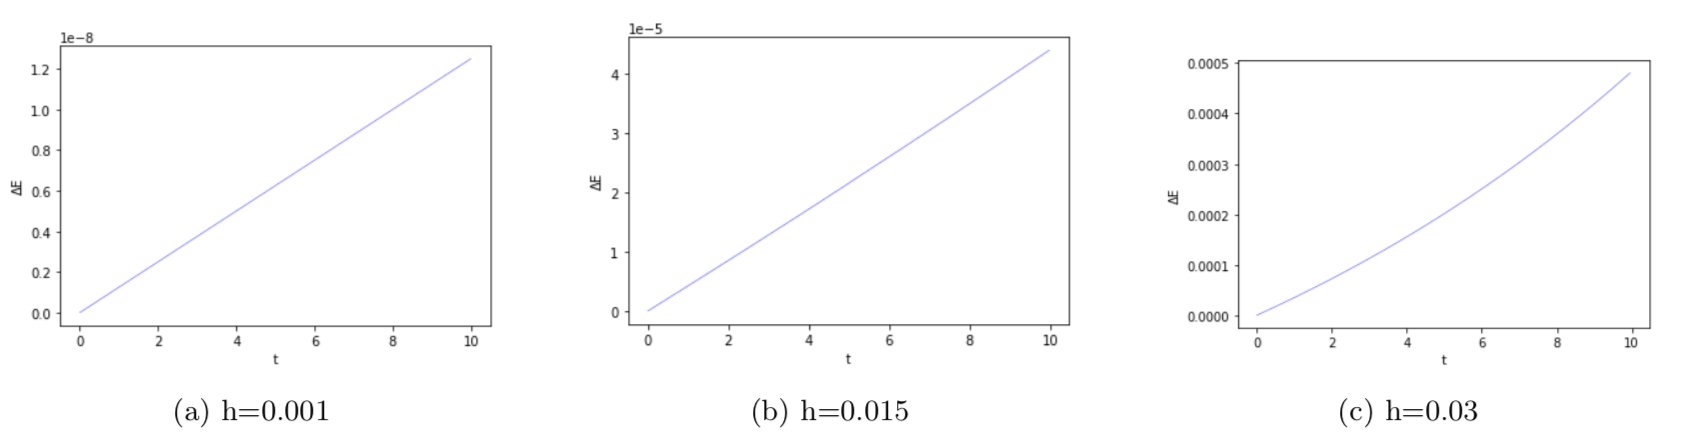
\includegraphics[width=18cm]{pic2.png}}
	\caption {Heun's method compared to analytical solution for different step sizes.}
\end{figure}
%
%
\begin{figure}[!h]
	\center{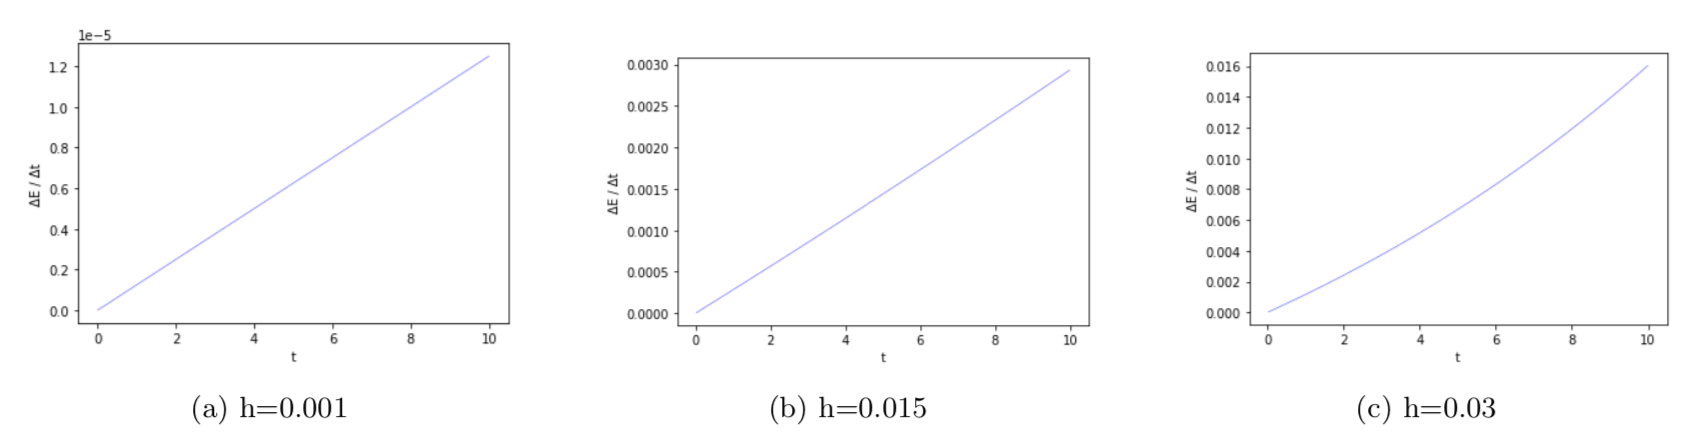
\includegraphics[width=18cm]{pic3.png}}
	\caption{$\Delta E / \Delta t$ for different timesteps.}
\end{figure}
%

\underline{\bf{Velocity-verlet method}}
\par The velocity-verlet method formally involves two evaluations of $f(x,t)$ per step:
\begin{equation}
   x(t + \Delta t) = x(t) + v \Delta t + \frac{a(t)} {a} \Delta t^2 
\end{equation}
%
\begin{equation}
   v(t) = v(t)  + \frac{a(t) + a(t + \Delta t)} {a} \Delta t 
\end{equation}
%
We start by looking at the phase space trajectory for both analytical and numerical solutions (ref fig.). From the phase space trajectory, we cannot really identify any deviation for different step sizes, but by looking at the position vs time and velocity vs time trajectories, we can see that numerical solution show small deviation for larger step size (ref fig 4).
%
%
\begin{figure}
\centering
\begin{subfigure}{.5\textwidth}
  \centering
  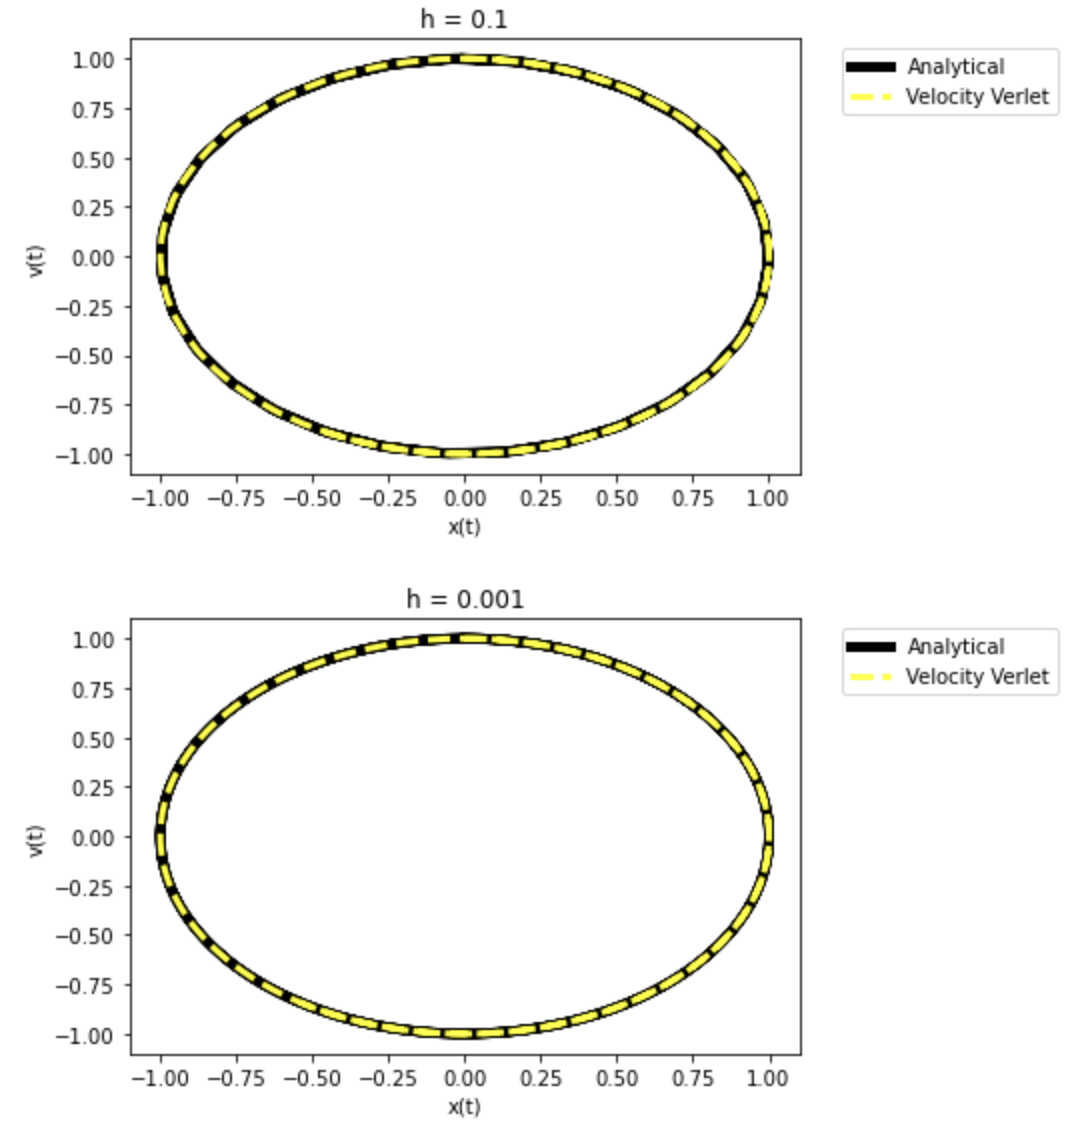
\includegraphics[width=.9\linewidth]{pic4.png}
  \caption{}
  \label{fig:sub1}
\end{subfigure}%
\begin{subfigure}{.5\textwidth}
  \centering
  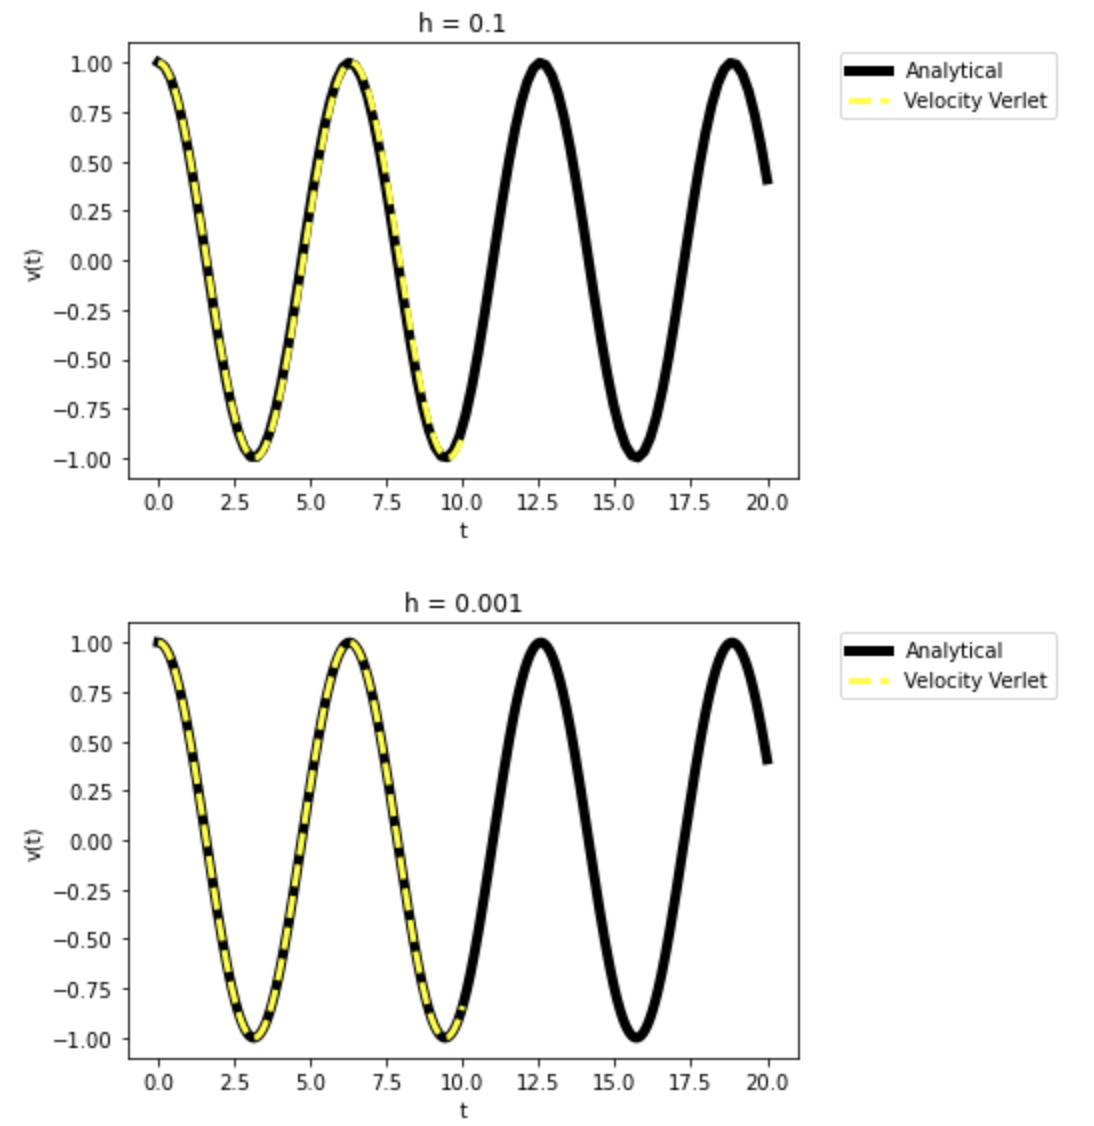
\includegraphics[width=.9\linewidth]{pic5.png}
  \caption{}
  \label{fig:sub2}
\end{subfigure}
\begin{subfigure}{.5\textwidth}
  \centering
  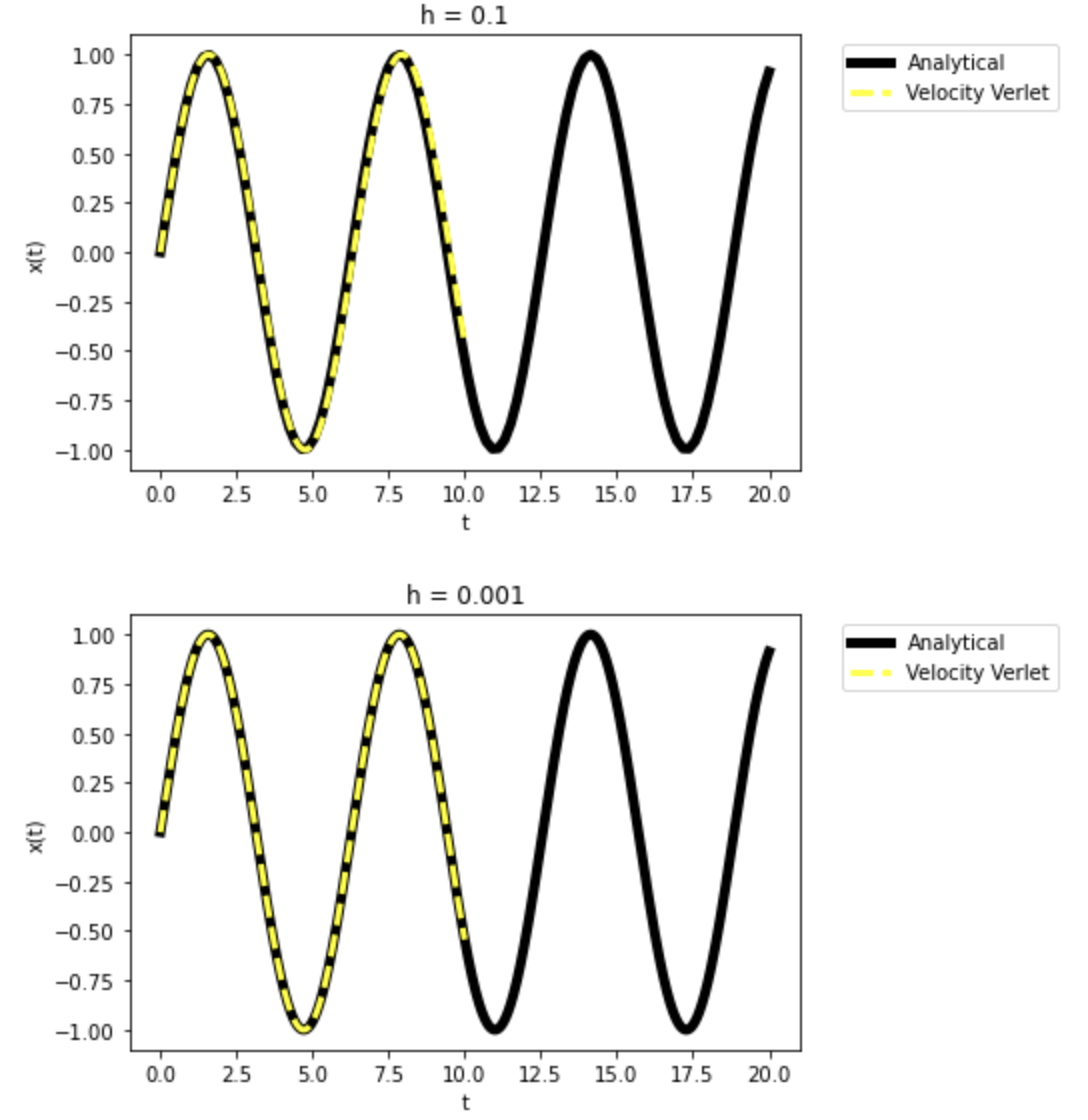
\includegraphics[width=.9\linewidth]{pic6.png}
  \caption{}
  \label{fig:sub3}
\end{subfigure}
\caption{}
\label{fig:test}
\end{figure}
%
%
\begin{figure}
\centering
\begin{subfigure}{.5\textwidth}
  \centering
  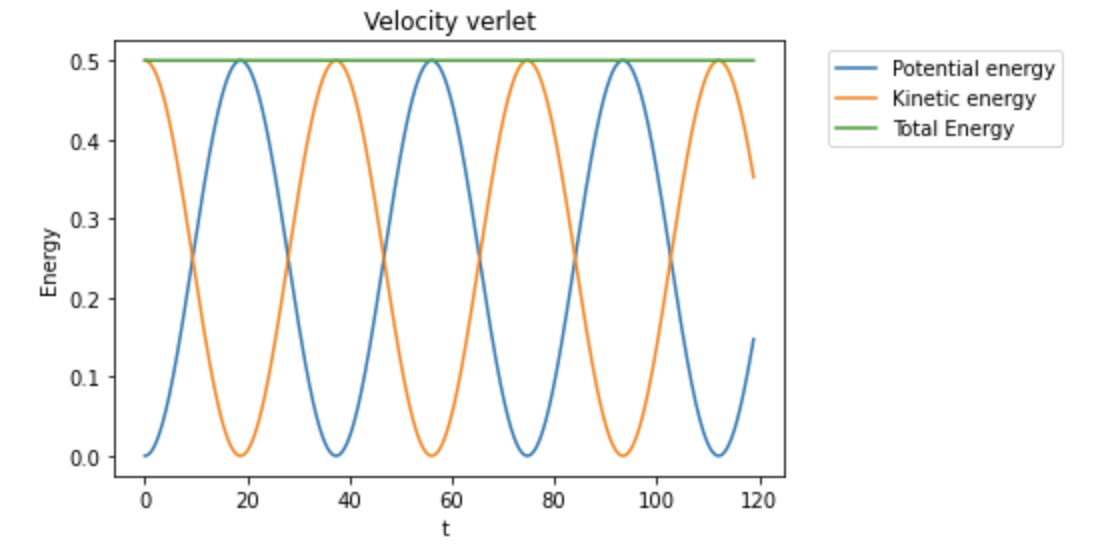
\includegraphics[width=.9\linewidth]{pic7.png}
  \caption{}
  \label{fig:sub1}
\end{subfigure}%
\begin{subfigure}{.5\textwidth}
  \centering
  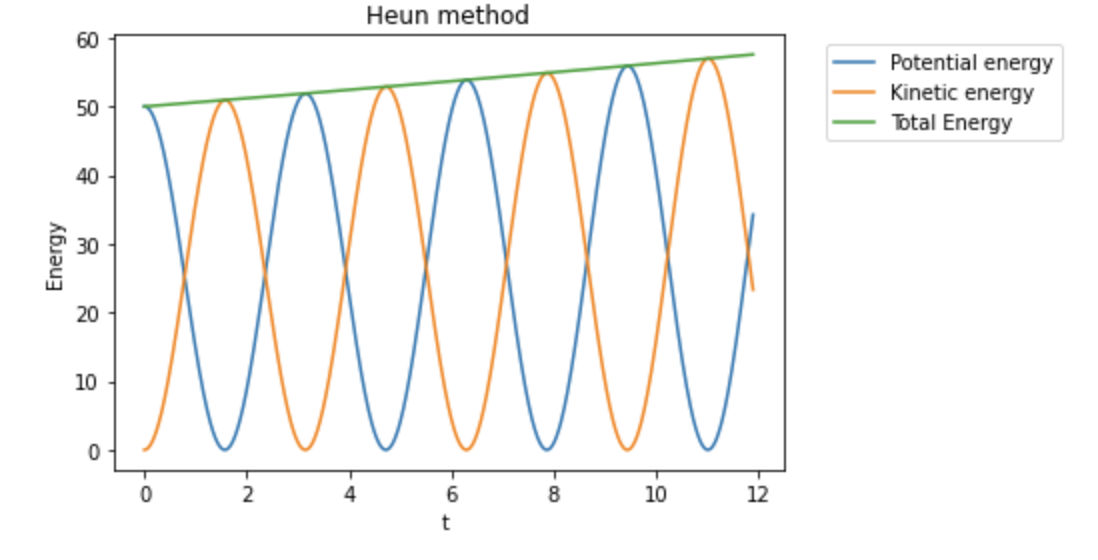
\includegraphics[width=.9\linewidth]{pic8.png}
  \caption{}
  \label{fig:sub2}
\end{subfigure}
\caption{Energy comparison of two methods. We can see that in velocity verlet method energy is constant and in Heun's method energy is increasing linearly with time. This makes the velocity verlet a good candidate for the molecular dynamics simulations.}
\label{fig:test}
\end{figure}
%

\end{s}
%
\begin{p}  Use your result from a) to compute the $n-th$ moment of a Gaussian
%
\begin{equation}
  
\end{equation}
%
%

%
\end{p}
	
\begin{s}

\begin{equation}
   \langle x^n \rangle = \begin{cases} 
   0,  & \text{for n = 2k+1} \\
   1,3,5, ... (n-1) & \text{for n=2k} 
\end{cases}
\end{equation}
%

%
\begin{equation}
 \langle x^n \rangle    = i^n  \frac{d^n G(k)}{dk^n} \bigg|_{k=0}
\end{equation}
%
In our case, characteristic function is,
%
\begin{equation}
     G(k)  = \int_{-\infty}^{\infty} dx   e^{-ax^2} e^{-ikx} 
\end{equation}
%
%
\begin{equation}
       = e^{-k^2 / 4a} \int_{-\infty}^{\infty} dx   e^{-a(x + \frac{ik}{2a})^2}  
\end{equation}

\begin{equation}
	G(k) =e^{-\frac{k^2} {4a}} \sqrt{\frac{\pi} {a}}
\end{equation}
%
Taking the log both sides,
%
\begin{equation}
	ln G(k) =-\frac{k^2} {4a}  + ln \left(\sqrt{\frac{\pi} {a}} \right)
\end{equation}
%
The second moment easily calculated by using the characteristic function,
%
\begin{equation}
	\langle x^2 \rangle = i^2 \frac{d^2} {dk^2} \left[ ln (\sqrt{\frac{\pi} {a} } ) - \frac{k^2} {4a} \right]
\end{equation}
%
%
\begin{equation}
	\langle x^2 \rangle = \frac{1}{2a}
\end{equation}
%
\end{s}
%%%%%%%%%%%%%%Second problem %%%%%%%%%%%%
\section{Fourier Transform}
















\end{document}
